\problemname{Räkneuttrycket}

Henning har fått i läxa att evaluera ett långt räkneuttryck. Det består av icke-negativa heltal åtskilda med operatorerna +, - och *. Han behöver dock inte använda sig av de gängse prioritetsreglerna, utan han kan fritt välja två närliggande tal med en operator emellan, evaluera detta uttryck och ersätta uttrycket med resultatet av operationen. Proceduren upprepas tills endast ett tal återstår: resultatet av evalueringen av hela uttrycket.

Skriv ett program som beräknar det största möjliga resultatet som kan erhållas.

\begin{figure}[ht!]
\centering
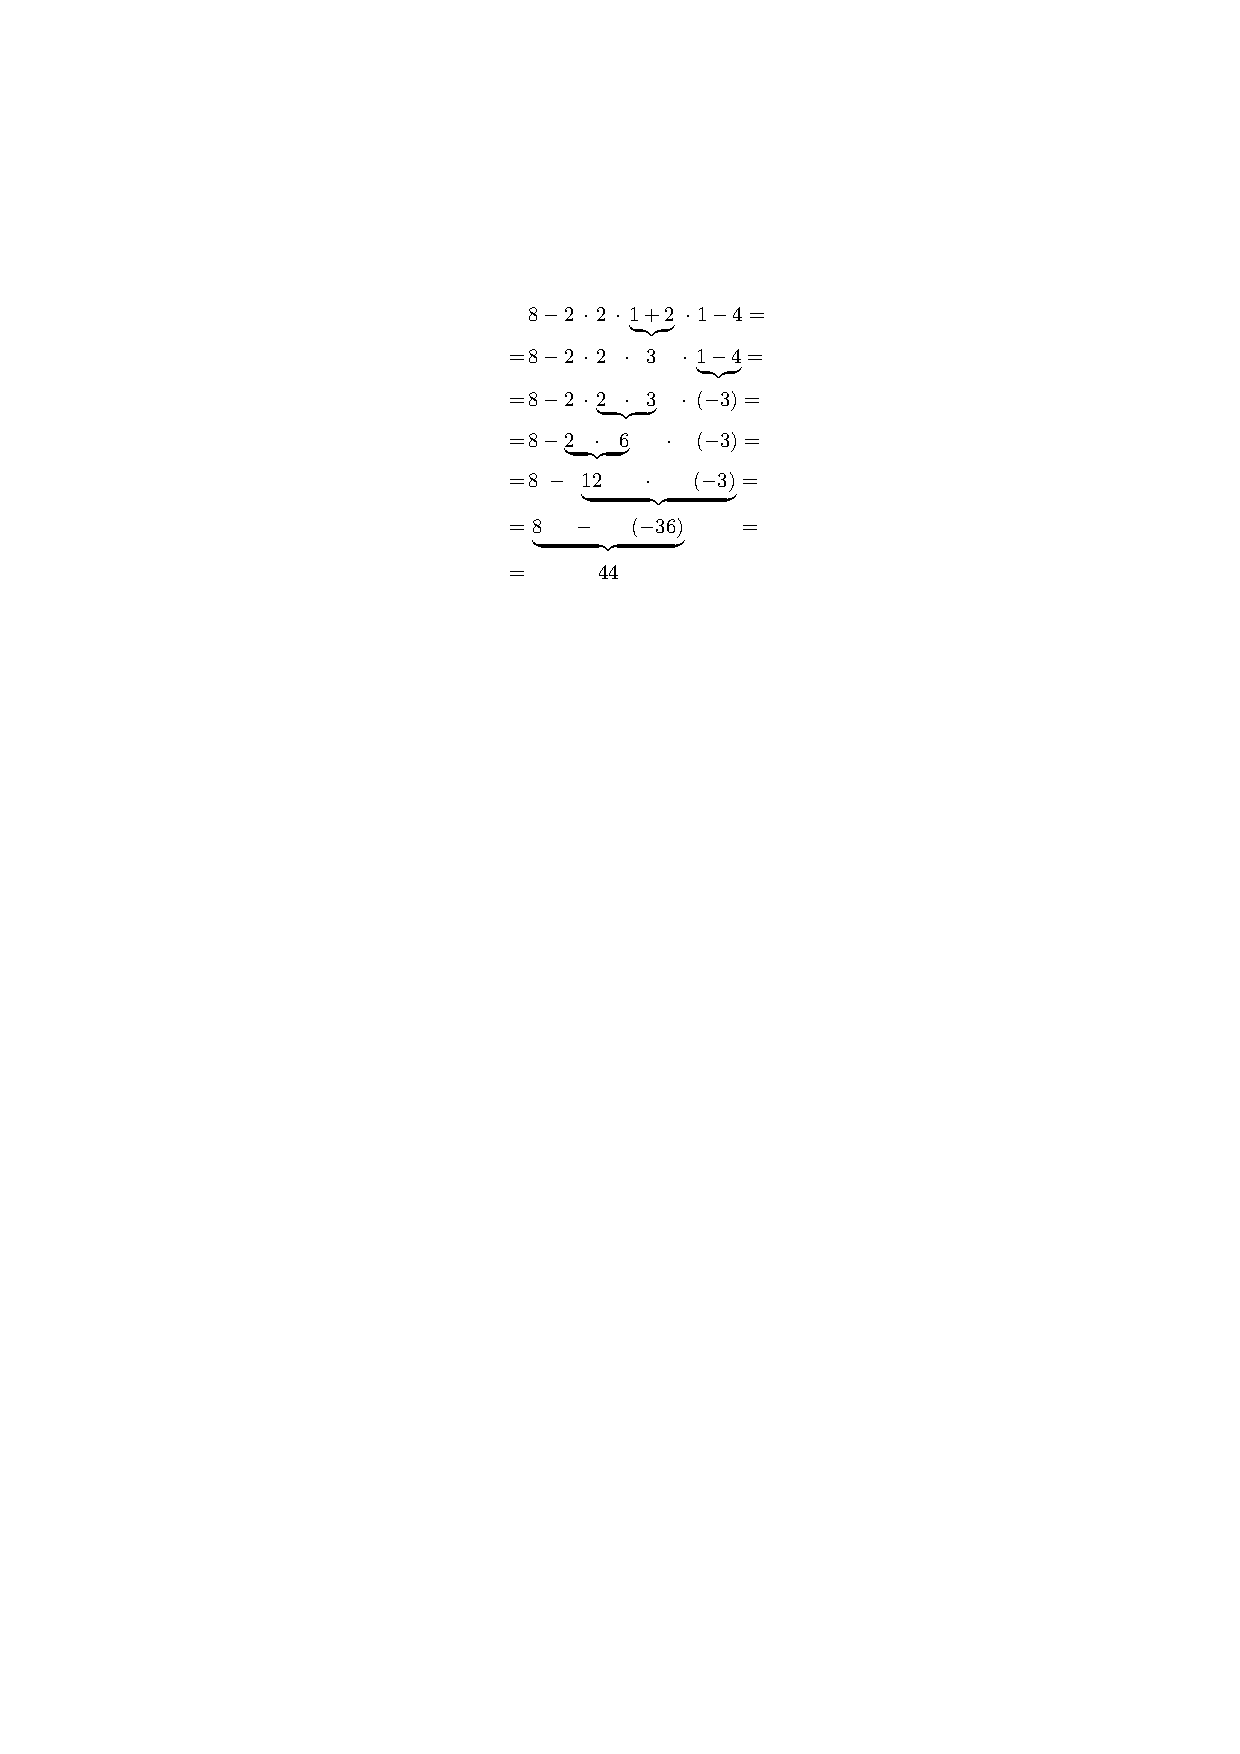
\includegraphics[width=0.4\textwidth]{example.pdf}
\caption{En optimal evalueringsordning i andra exemplet.}
\label{overflow}
\end{figure}

\section*{Input}

På första raden står en sträng med max 100 tecken: uttrycket som ska evalueras. Det följer mönstret [tal] [operator] [tal] [operator]....[operator] [tal] utan några blanksteg. Varje operator är antingen +, - eller * och varje ingående tal $k_i$ uppfyller $0\leq k_i < 1000000$. Inget tal skrivs med överflödiga inledande nollor.

\section*{Output}

Ett heltal: det största värdet som kan erhållas genom att evaluera uttrycket i valfri ordning. Detta tal, liksom alla möjliga delresultat som kan uppkomma, är alltid större än $-10^{18}$ och mindre än $10^{18}$.


\section*{Poängsättning}
Din lösning kommer att testas på flera testfallsgrupper. För att få poäng för en grupp
så måste du klara alla testfall i gruppen.

\begin{tabular}{| l | l | l |}
\hline
Grupp & Poängvärde & Gränser \\ \hline
1     & 11         & Endast operatorerna + och * förekommer. Antalet tal är högst 10 och de uppfyller $1\leq k_i \leq 9$. \\
2     & 11         & Alla operatorer förekommer. Antalet tal är högst 10. \\
3     & 37         & Endast operatorerna + och * förekommer.\\ 
4     & 41         & Alla operatorer förekommer. \\ \hline
\end{tabular}


